\chapter{Návrh aplikace}
    Návrh aplikace je velice důležitou fází projektu, ve které by mělo dojít ke sjednocení požadavků zadavatelů a reálného provedení. Vytvořením dobrého návrhu se zamezí případným kolizím a zároveň proběhne první interakce mezi zákazníkem a dodavatelem. Ze strany UČL byl vznesen požadavek, aby aplikace byla snadno ovladatelná a měla moderní vzhled. Databázové schéma bylo čistě na mém rozhodnutí.
    
    \section{Wireframy}

        Jednou z nejdůležitějších sekcí bylo navrhnout, jak budou jednotlivé stránky vypadat a kolik jich aplikace bude obsahovat. Základní rozložení stránek bylo na mém rozhodnutí, nicméně musel jsem dodržet požadavky UČL AV. Design měl být jednoduchý, uživatelsky přívětivý a moderní. Tyto návrhy musely být a byly schváleny pracovníky UČL AV.
        
        Grafika měla být jednoduchá, bez složitých a obsáhlých prvků. Pro snadnější a moderní stylování aplikace byl použit Bootstrap\footnote{domovská stránka: \url{https://v4-alpha.getbootstrap.com/}}. Jedná se o volně dostupnou knihovnu, která dovoluje stylovat vzhled aplikace pouze přídáním určitých tříd k elementům. Při dodržování pravidel Bootstrapu není potřeba vkládat obsáhlé CSS styly. Pomocí Bootstrapu lze poměrně snadno vytvořit responzivní aplikaci. Toho by se dalo využít v případém budoucím rozšíření.
        
        Pro návrh GUI jsem se rozhodl použít webovou aplikaci Moqups\footnote{domovská stránka: \url{https://moqups.com/}}. Její bezplatná verze nabízí obrovské množství šablon pro grafické návrhy. Od základních prvků jako je tlačítko nebo nadpis, po mírně složitější formuláře. Je velikou výhodou, že Moqups má v nabídce prvky Bootstrapu . 
        
        \subsection{Login}
            Pro úvodní přihlašovací stránku jsem vybral jednoduchý formulář, ve kterém je email a heslo, viz obrázek \ref{fig:login}. Pozadí, které by se dalo v budoucím rozšíření měnit, je jako na všech ostatních stránkách bílé.
            
        \subsection{Hlavní stránka}
            Po úspěšném přihlášení do aplikace se zobrazí hlavní stránka, která je rozdělena do tří částí, jak je vidět na obrázku \ref{fig:main}. V hlavičce se nachází společně s nadpisem odkaz na seznam autorů a vydavatelů děl a dropwdown s možnostmi uživatele. Dále je zde filtr aplikovatelný na zobrazená díla. Zadání vyžadovalo vyhledat elektronickou literaturu podle autora, roku vydání, textu obsaženého v díle a statusu. Třetí část obsahuje samotný seznam děl. Tento seznam je ve tvaru tabulky se sloupci název díla, autor, rok vydání, status, odkaz na přílohy a nezbytné akce a navíc se dá tabulka seřadit podle sloupců. U seznamu děl lze nastavit počet zobrazených děl a obsahuje rychlý vyhledávač textu.

        \subsection{Metadata}
            Na obrázku \ref{fig:metadata} je vidět rozložení stránky pro úpravu základních údajů o dílu. Opět se skládá ze tří částí. První obsahuje navigaci, dropdown pro přihlášeného uživatele a nadpis. Druhá část je věnována autorům a vydavatelům. V tomto oddílu bude umožněno přidávat a odebírat autora nebo vydavatele. Poslední sekce obsahuje formulář pro úpravu metadat literárního díla. Společně s pracovníky UČL AV byly vybrány nejdůležitější atributy, které je zde možno upravit. 
        
        \subsection{Přílohy}
            Součástí zadání práce je správa příloh, zejména fotografií. Přílohám se věnuje právě tento segment. Obsahem wireframu \ref{fig:attachments} jsou naskenované jednotlivé stránky daného literárního díla. V horní části se opět objevuje navigace, uživatelské funkce a nadpis. Následuje sekce věnovaná hromadnému uploadu skenů do níže zobrazené fotogalerie.
            
        \subsection{Autoři a vydavatelé}
            Pro správu autorů a vydavatelů byl použit návrh zobrazený v příloze \ref{fig:authPub}. V horní části se vyskytuje navigace, nezbytné funkce a nadpis. Dále je zde umístěna tabulka záznamů, ve kterých lze snadno vyhledávat. Každý záznam lze upravit a smazat. Pro upravení záznamu byl navržen wireframe \ref{fig:edit}, který obsahuje navigaci, funkce a zjednodušený formulář. Formuláře pro upravení vydavatele nebo autora jsou totožné.
            
            \begin {figure}[H]\centering
                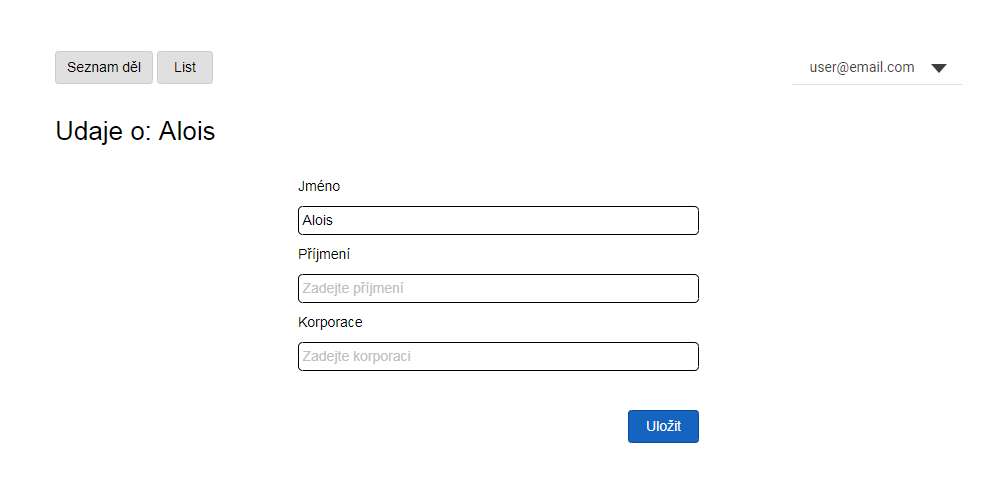
\includegraphics[width=\textwidth]{images/edit}
                \caption {Úprava autora}
                \label {fig:edit}
            \end{figure}
            
        \subsection{Text}
            Nejdůležitějším prvkem aplikace byla bezesporu možnost upravovat text literárního díla. Pro tuto funkci byla navržena stránka \ref{fig:text}. Jako u předešlých wireframů, horní část se věnuje navigaci, funkcím uživatele a nadpisu. Dále je vidět rozložení stránky na dva oddíly. Jeden pro text knihy a druhý pro možnost vkládání značek. Menu vpravo bylo navrženo vzhledem k nadměrné velikosti první části tak, aby bylo viditelné, když se uživatel posune níž.
            
    \section{Databázové schéma}
        Neméně duležitou součástí projektu byla databáze. Ze strany UČL AV nebyly vzneseny žádné požadavky na podobu databáze, proto se mohlo schéma přizpůsobit dle potřeby aplikace.
        
        Pro model databáze byla použita webová aplikace\footnote{domovská stránka: \url{https://www.quickdatabasediagrams.com/}}. Schéma je navrženo minimalisticky, ale tak aby zároveň pokrývalo veškeré potřeby aplikace. Výsledný návrh databáze \ref{fig:schema} obsahuje 5 tabulek s jednoduchými vazbami.
        
        \begin {figure}[H]\centering
            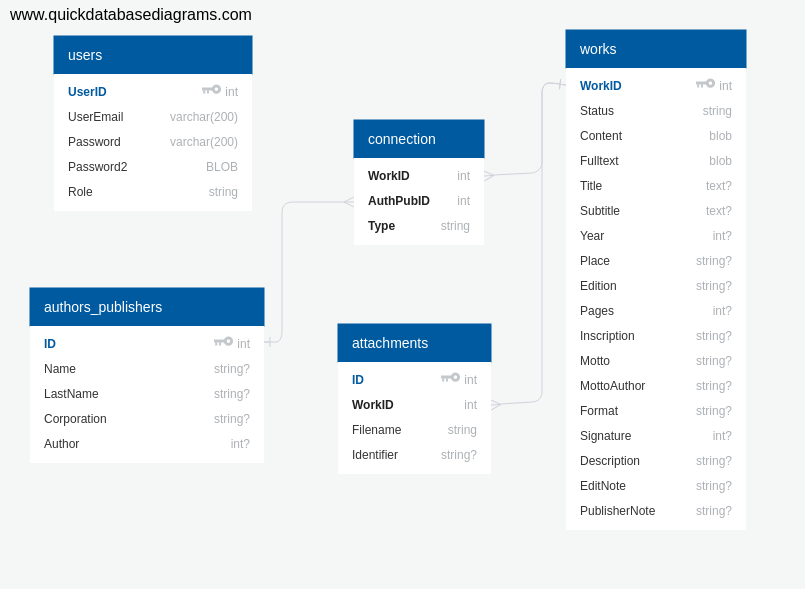
\includegraphics[width=\textwidth]{images/schema}
            \caption {Databázové schéma}
            \label {fig:schema}
        \end{figure}
        
        V tabulce uživatelů je uloženo UserID, UserEmail a heslo rozdělené do dvou sloupečků viz \ref{autentizace}. Uživatelské role jsou identifikovány pomocí sloupce Role.
        
        Duležitá tabulka je connection. Obsahuje reference na tabulky works a authors\_publishers. Třetím atributem je typ spojení. Tento typ určuje, jestli je spojením autor nebo vydavatel. Každý záznam v tabulce propojuje dílo a autora nebo vydavatele. Primárním klíčem je celá trojice, to znamená, že v tabulce se nemohou vyskytovat duplicity.
        
        ID, Name, LastName, Corporation a Author jsou atributy tabulky authors\_publishers. Záznamem může být reálná osoba, její pseudonym nebo společnost. V případě pseudonymu odkazuje záznam na reálnou osobu. Tuto referenci obsahuje sloupec Author, ve kterém je ID reálné osoby zaznamenané v authors\_publishers nebo je prázdný.
        
        Nejobsáhlejší tabulka se nazývá works. Obsahuje všechny základní informace o dílu: název díla (Title), podtitul (Subtitle), datum publikace (Year), místo vydání (Place), pořadí vydání (Edition), počet stran sbírky (Pages), věnování autora (Inscription), motto (Motto), autor motta (MottoAuthor), formát naskenovaného díla (Format), podpis (Signature), popis díla (Description) a poznámka k vydání (EditNote). Ve works je atribut Status, který indikuje momentální stav díla. Status může nabývat hodnot Nové, Rozpracováno, Zkontrolováno a Hotovo. Celý text včetně tagů je ve sloupci Content. Dále tabulka works obsahuje sloupec Fulltext, ve kterém je text díla bez tagů.
        
        Poslední tabulka attachments je pro přílohy přidružené k dílům. Obsahuje ID, referenci na dílo, Filename a poznámku k obrázku (Identifier).
        
    \section{Autentizace} \label{autentizace}
        Součástí zadání je autentizace. Ze strany ústavu nebyl vznesem žádný požadavek na ochranu hesel, proto jsem si způsob šifrování mohl vybrat. Heslo je zašifrované pomocí sha256. Pro větší bezpečnost hesla jsem přidal metodou solení hesla tzn., že se k uživatelskému heslu přidává náhodný text.
        
